\subsection{Data Representation}
\label{sec:asttheory}
Here is an example of how the \textit{top-down} parsing algorithm works, demonstrated with an AST.

\begin{figure}[H]
\begin{center}
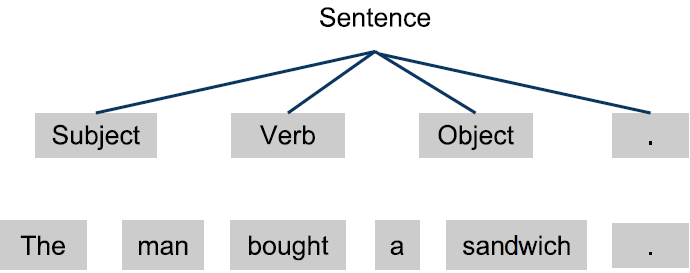
\includegraphics[scale=0.5]{Images/parsingexample/AST1.png}
\end{center}
\caption{The first step for the parser is to decide what to apply ind the root node. Here it has only one option: "Sentence ::= Subject Verb Object."}
\end{figure}

The words that are not shaded are final elements in the AST. The words that are shaded and has a line to the previous node, is called stubs, and are not final elements, because they depend on the terminal nodes. The shaded nodes with no connection lines are the terminal symbols that are not yet examined.

\begin{figure}[H]
\begin{center}
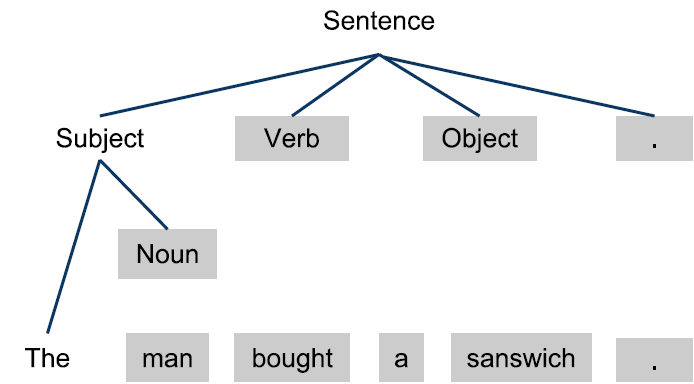
\includegraphics[scale=0.5]{Images/parsingexample/AST2.png}
\end{center}
\caption{In the second step the parser looks at the stub to the left. Here the correct production rule is: "Subject ::= \textbf{The} noun".}
\label{fig:ast2}
\end{figure}

The parser chooses the production rules by examining the next input terminal symbol. If the terminal symbol in figure \ref{fig:ast2} had been "A" then it would have chosen the production rule: "Subject ::= \textbf{A} noun".

\begin{figure}[H]
\begin{center}
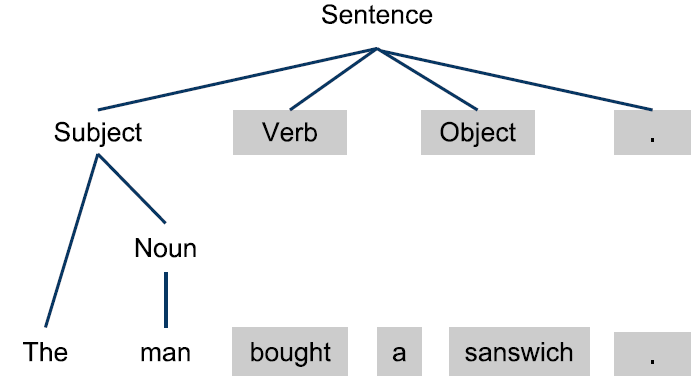
\includegraphics[scale=0.5]{Images/parsingexample/AST3.png}
\end{center}
\caption{In third step the noun-stub is concidered, and the production rule becomes: "Noun ::= man".}
\end{figure}

\begin{figure}[H]
\begin{center}
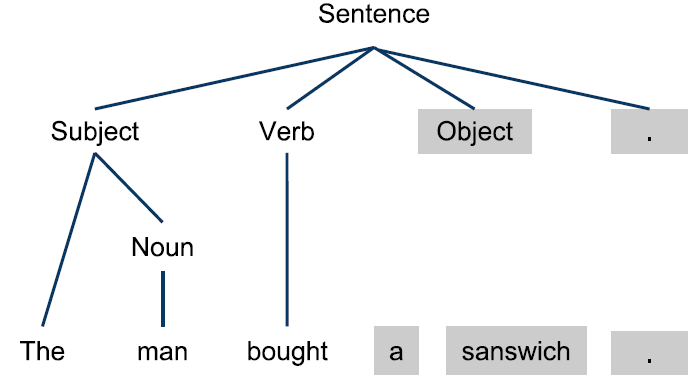
\includegraphics[scale=0.5]{Images/parsingexample/AST4.png}
\end{center}
\caption{In fourth step the verb-stub is concidered, and the production rule becomes: "Verb ::= bought".}
\end{figure}

\begin{figure}[H]
\begin{center}
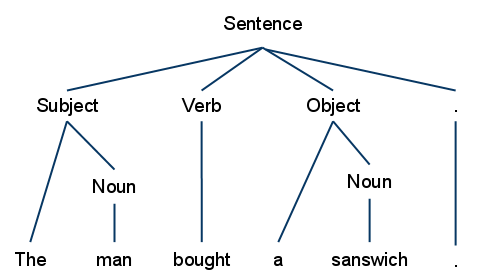
\includegraphics[scale=0.5]{Images/parsingexample/AST5.png}
\end{center}
\caption{Here is the final syntax tree when the parser is done.}
\end{figure}

This method is continued until the whole sentence has been parsed. Here the final syntax tree is quite simpel, but one can imagine how the tree will grow when the input is a larger program text. See section \ref{AST} on how we have implemented the AST.